\chapter{Caracterización del  Electroimán} \chapterlabel{Informe/3-CaracterizacionElectroiman} \label{cap:CaracterizacionElectroiman}

\noindent El objetivo de este apartado es poder obtener un modelo físico del electroimán que se dispone. A partir de sus características constructivas, se determinarán otros parámetros del sistema de control (como masa máxima, corriente nominal de trabajo, etc)


\section{Modelado físico}


%\section{Caracterización del Electroimán}

%\noindent El actuador de este sistema de control es un electroimán. Se eligió construirlo utilizando un núcleo de acero al silicio con un bobinado en su interior. 
%mejorar esto

\noindent Se puede modelar el sistema como un objeto de masa puntual que es sometido a dos fuerzas opuestas en el eje “Y” de la figura \ref{fig:img_modelado-fisico}: la de su propio peso hacia abajo, y una fuerza realizada por el electroimán en sentido contrario. \colorbox{red}{MARCAR Yo EN LA IMAGEN}

%capaz poner otra imagen
\begin{figure}[H]
	\centering
	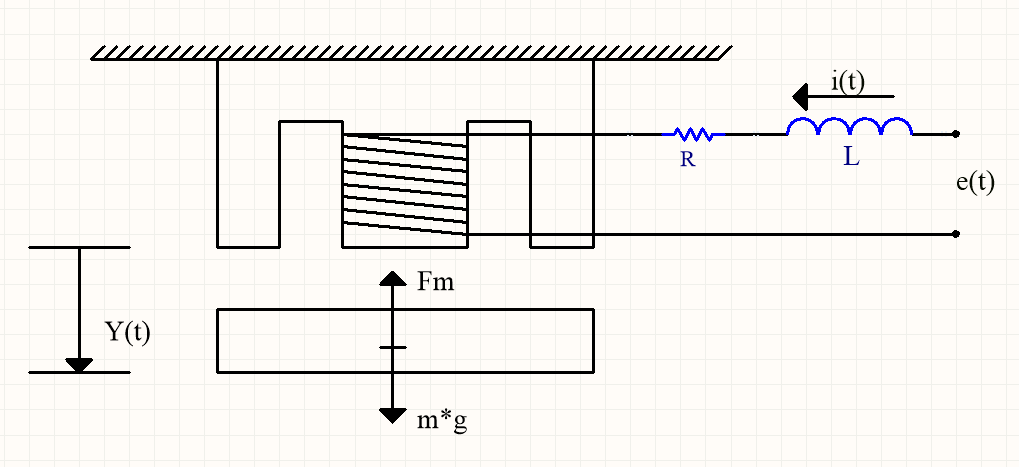
\includegraphics[width=\textwidth]{modelo-fisico.png}
	\caption{Modelado físico.}
	\label{fig:img_modelado-fisico}
\end{figure}

\noindent La fuerza correspondiente al peso del objeto es $P=m*g$, donde $m$ es la masa en kg y $g$ es la aceleración de la gravedad en $\frac{m}{s^{2}}$. Para mantenerlo levitando en estado de equilibrio, el electroimán debe generar una fuerza de igual módulo y sentido contrario. Esto lo logra a partir de la circulación de un flujo magnético entre su núcleo y la pieza con forma de I. Entre estas dos piezas se conforma lo que se conoce como circuito magnético, en el que la energía fluye impulsada por una fuerza magnetomotriz.

%hacer una intro de como se genera la fuerza magnética???
\noindent La fuerza magnetomotriz generada en el núcleo del electroimán es proporcional a la corriente que circula por su bobinado, y su módulo está dado por la ecuación \ref{eq_fuerza-magnetomotriz}, que también la relaciona con la reluctancia del circuito magnético y la magnitud del flujo magnético.

\begin{equation} \label{eq_fuerza-magnetomotriz}
	F_{mm}=N*i=R_{m}*\phi	
\end{equation}

%mejorar este parrafo
\noindent $R_{m}$ corresponde a la reluctancia del circuito magnético, $\phi$ indica la magnitud del flujo, es decir, la cantidad de campo magnético que atraviesa una superficie y $F_{mm}$ es la fuerza magnetomotriz (que es distinta a la fuerza magnética $F_{m}$). La ley de Hopkinson relaciona estos parámetros con la corriente que circula por el bobinado ($i$) y la cantidad de vueltas de su núcleo ($N$).


\noindent Por otro lado, la inductancia del bobinado está dada por la ecuación \ref{eq_inductancia_flujo}

\begin{equation} \label{eq_inductancia_flujo}
	L*i=N*\phi
\end{equation}


\noindent El electroimán utilizado (figura \ref{fig:img_modelado-fisico}) está compuesto por una pieza en forma de E y otra en forma de I, que se encuentran separadas por un espacio o gap de aire. Este circuito magnético se puede modelar como a un toroide con un corte o separación  de longitud $lA=2*y_{o}$, como se muestra en la figura \ref{fig:img_toroide}

\begin{figure}[H]
	\centering
	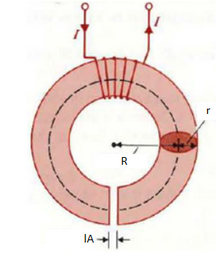
\includegraphics[scale=0.75]{toroide.png}
	\caption{Toroide con gap de aire.}
	\label{fig:img_toroide}
\end{figure}

\noindent Partiendo del caso de un toroide sin gap de aire, se puede modelar su reluctancia con la ecuación \ref{eq_reluctancia}. En la que A es el área transversal, $\mu_{r}$ es la permeabilidad relativa del material, $\mu_{o}$ es la permeabilidad magnética en el vacio y $l_{h}$ es la longitud del circuito magnético. 

\begin{equation}\label{eq_reluctancia}
	R_{m}=\frac{l_{h}}{\mu_{o}*\mu_{r}*A}
\end{equation}

\noindent Combinando las ecuaciones \ref{eq_fuerza-magnetomotriz}, \ref{eq_inductancia_flujo}, y \ref{eq_reluctancia}, se llega a la expresión de la inductancia del toroide sin gap de aire:

\begin{equation}\label{eq_inductancia}
	L=\frac{N}{i}*\phi=\frac{N}{i}*\frac{N*i}{R_{m}}=\frac{N^	{2}*A*\mu_{o}*\mu_{r}}{l_{h}}
\end{equation}


\noindent Al agregar un gap de aire, se genera una discontinuidad en el medio magnético de distancia $l_{A}$ (longitud en el aire).

\noindent El flujo magnético atraviesa esta discontinuidad sin desviaciones (siempre que $l_{A}$ sea pequeña comparada con el área transversal A).

\noindent Al haber un gap de aire la reluctancia del sistema aumenta, por lo que se debe sumar, en serie a $R_{m}$, la reluctancia en el aire $R_{a}$. Por otro lado, $l_{h}$ prácticamente no se ve modificada ya que es una pequeña incisión en el circuito magnético. De esta forma, se obtiene la ecuación \ref{eq_inductancia_con_gap}.

\begin{equation}\label{eq_inductancia_con_gap}
L=\frac{N^{2}}{R_{m}*R_{a}}=\frac{N^{2}}{\frac{l_{h}}{A*\mu_{o}*\mu_{r}}+\frac{l_{a}}{A*\mu_{o}}}=\frac{N^{2}*A*\mu_{o}}{l_{a}+\frac{l_{h}}{\mu_{r}}}
\end{equation}

\noindent Debido a que $l_{a}$ es el gap de aire, se debe reemplazar por la distancia de separación entre las dos piezas magnéticas, que está representada por la variable $y_{o}$. En el caso de nuestro electroimán, las líneas de fuerza atraviesan dos veces y, por lo tanto $l_{a}=2*y_{o}$.

\noindent Además, en la ecuación \ref{eq_inductancia_con_gap} $\mu_{r}>>1$ entonces $2*y_{o}>>\frac{l_{h}}{\mu_{r}}$, se obtiene la inductancia en función de la distancia del gap de aire:

\begin{equation}\label{eq_inductancia_vs_y}
		L(y)=\frac{{N^{2}*A*\mu_{o}}}{2*y_{o}}
\end{equation}

\section{Cálculo de la fuerza magnética}

\noindent La fuerza magnética de atracción que ejerce el electroimán sobre la pieza en forma de I se puede modelar a partir de la energía almacenada en un inductor y al considerar que esta es igual al trabajo:

\begin{equation}\label{eq_energia}
	E(i,y)=W=\int{F_{m}*dy}=>F_{m}=\frac{\partial{E(i,y)}}{\partial{y}}
\end{equation}

\noindent Siendo $E(i,y)$ la energía que almacena un inductor en su campo magnético:

\begin{equation}\label{eq_energia_2}
	E(i,y)=\frac{L(i,y)*i^{2}}{2}
\end{equation}

\noindent La expresión anterior indica que la cantidad de energía que almacena el sistema es función del gap de aire ($y$) y de la corriente que circula por el electroimán ($i$). Combinando las ecuaciones \ref{eq_inductancia_vs_y}, \ref{eq_energia} y \ref{eq_energia_2}:

\begin{equation}\label{eq_fuerza_magnetica}
	\abs{F_{m}}=\frac{\partial{E(i,y)}}{\partial{y}}=\frac{i^{2}}{2}*\frac{\partial{\frac{{N^{2}*A*\mu_{o}}}{2*y}}}{\partial{y}}=\frac{i^{2}*N^{2}*\mu_{o}*A}{4*y^{2}}
\end{equation}

\noindent Como se puede apreciar en la ecuación \ref{eq_fuerza_magnetica} la fuerza es proporcional al cuadrado de la acción de control (es decir, de la corriente), e inversamente proporcional al cuadrado de la variable que se desea controlar (es decir, de la distancia). Por lo tanto, el problema adquiere un comportamiento no lineal.

\section{Diseño del electroimán}

\noindent El electroimán está construido por un núcleo de acero laminado con forma de E, que tiene un cable bobinado en su rama central, y otra pieza con forma de I.\colorbox{red}{poner imagen con dimensiones}. 
% 

Está construido por una laminación normalizada sin desperdicio 600. Estas son útiles ya que cada par de laminas E y I puede fabricarse a partir de una lámina de acero rectangular, de manera de que no se desperdicia material durante la fabricación. \colorbox{red}{poner figura}

Está compuesto por dos piezas: una con forma de “E” y otra con forma de “I”. En su núcleo tiene un bobinado de 150 vueltas (N) de cobre esmaltado con un diámetro de $2.5$ mm. El núcleo es de sección cuadrada ya que esto maximiza el área mientras que disminuye el perímetro, reduciendo así la longitud media de las espiras y ahorrando material. 

\section{Análisis del electroimán}

\noindent El electroimán del que se dispone tiene las siguientes características:
asd
asd
qwe


\noindent En base a estos datos podemos determinar otras variables del sistema como son: masa máxima, distancia máxima de separación, corriente nominal de trabajo.

%\noindent Se debe determinar qué dimensiones debe tener el electroimán a utilizar para que sea capaz de ejercer la fuerza magnética necesaria para mantener levitando el peso deseado.

%\noindent Al analizar la ecuación \ref{eq_fuerza_magnetica} se puede observar que hay dos parámetros que son propios del electroimán: el área del núcleo A y la cantidad de vueltas del bobinado N. 

\noindent Para obtener una expresión de diseño, partimos de la ecuación \ref{eq_fuerza_magnetica} y la igualamos a la fuerza ejercida por el peso del objeto que se debe hacer levitar ($\abs{F_{m}}=m*g$):

\begin{equation}\label{eq_fuerza_peso}
	m*g=\frac{i^{2}*N^{2}*\mu_{o}*A}{4*y^{2}}
\end{equation}

\noindent De la ecuación \ref{eq_fuerza_peso}, y a partir de las condiciones de diseño del problema, se puede determinar la corriente necesaria para mantener el objeto en suspensión:

\begin{equation} \label{eq_corriente_peso}
	i_{nom}=\sqrt{\frac{4*m*g*y^{2}}{N^{2}*\mu_{o}*A}}
\end{equation}

Considerando las condiciones mas exigentes para el sistema, con $m=m_{max}=30kg$ e $y=y_{max}=5mm$:

\begin{equation}
	i_{nom}=20.4A
\end{equation}

\noindent Aunque esta corriente es suficiente para mantener el objeto en estado de equilibrio, se necesita una corriente mayor para poder responder ante perturbaciones en la distancia de separación, por lo tanto se define la corriente máxima $i_{max}=30A$.



\section{Expresión de inductancia linealizada}

\noindent Volviendo a la ecuación \ref{eq_inductancia_vs_y}, se realiza una expansión por serie de Taylor y se desprecian los términos de orden mayor o igual a 2, con el objetivo de llegar a una expresión lineal para la inductancia se obtiene:

\begin{equation} \label{eq_inductancia_lineal_teorica}
	L(y)[mH]=-2.2089*y[mm]+17.67 [mH]
\end{equation}

\section{Mediciones sobre el electroimán}

\colorbox{red}{esto iría acá??}

\section{Modelo de estado de la planta}

\noindent Al plantear un diagrama de cuerpo aislado del sistema \colorbox{red}{poner imagen} y plantear la sumatoria de fuerzas en el eje y:

\begin{equation}\label{eq_sumatoria_fuerzas_y}
	\sum F_{y}=m*a=>m*g-F_{m}=m*\ddot{y}
\end{equation}

\noindent De la ecuación \ref{eq_fuerza_magnetica} se convierte la ecuación \ref{eq_sumatoria_fuerzas_y} en:

\begin{equation}\label{eq_sumatoria_fuerzas_y_2}
	m*\ddot{y}=m*g-K*\frac{i(t)^{2}}{y(t)^{2}}
\end{equation}

\noindent Donde K es una constante de valor:

\begin{equation}
	K=\frac{N^{2}*\mu_{o}*A}{4}=1.77*10^{-5} [\frac{N*m^2}{A^2}]
\end{equation}

\noindent Teniendo en cuenta que $i(t)$ es la entrada a la planta, se puede plantear un modelo con las siguientes variables de estado:\newline
\colorbox{red}{se puede poner mas grande??}
\begin{equation}
	x_{1}=y(t)
\end{equation}
\begin{equation}
	x_{2}=\dot{x_{1}}
\end{equation}
\begin{equation}
	u=i(t)
\end{equation}

\noindent Por lo tanto se obtienen dos ecuaciones de estado:

\begin{equation}
	\dot{x_{1}}=x_{2}
\end{equation}
\begin{equation}
	\dot{x_{2}}=g-\frac{K}{m}*\frac{u^{2}}{x_{1}^{2}}
\end{equation}

El modelo es no lineal, por lo tanto se utiliza el método de linealización por serie de Taylor. En primer lugar se deben encontrar los puntos de equilibrio del sistema; por las condiciones del problema se define $x_{1o}=4mm$. El resto de los puntos de equilibrio se encuentrar igualando las derivadas a cero:
\begin{equation}
	x_{1o}=4mm
\end{equation}
\begin{equation}
	x_{2o}=0
\end{equation}
\begin{equation}
	u_{o}=\sqrt{\frac{m*g}{K}}*x_{1o}
\end{equation}

Por lo tanto las ecuaciones linealizadas quedan:

\begin{equation}
	\dot{x_{1}}=x_{2}
\end{equation}

\begin{equation}
	\dot{x_{2}}=2*\frac{K*u_{o}^{2}}{m*x_{1o}^{3}}*x_{1}-2*\frac{K*u_{o}}{m*x_{1o}^{2}}*u
\end{equation}

Las matrices del modelo quedan:

\begin{equation}
	A=\begin{bmatrix}
		0 & 1\\
		\frac{2*g}{y_{o}} & 0
	\end{bmatrix}
\end{equation}

\begin{equation}
	B=\begin{bmatrix}
		0\\
		-\frac{2}{y_{o}}*\sqrt{\frac{K*g}{m}}
	\end{bmatrix}
\end{equation}

\begin{equation}
	C=\begin{bmatrix}
		1 & 0\\
	\end{bmatrix}
\end{equation}

\noindent Es posible obtener la función transferencia de la planta utilizando:

\begin{equation}\label{eq_transferencia_planta}
	G_{planta}=C*(S*I-A)^{-1}*B
\end{equation}

\noindent Finalmente, se obtiene para $m=30kg$ e $y_{o}=4mm$:

\begin{equation}
	G_{planta}=-\frac{2}{y_{o}}*\frac{\sqrt{\frac{K*g}{m}}}{S^2-\frac{2*g}{y_{o}}}=\frac{-1.201}{S^{2}-4900}
\end{equation}

\noindent La planta tiene dos autovalores en $+-\sqrt{\frac{2*g}{y_{o}}}=+-70[\frac{rad}{s}]$. Es decir, uno en el semiplano izquierdo y otro en el derecho, lo que provoca que la planta sea inestable y se deba buscar una estrategia de control apropiada para controlarla.
